\chapter{Spatial Discretization}\label{chap.discrete}
%===================================================================

%--------------------------------------------------------------------
\section{Foreword}

The original explicit version of GYRO has been partially 
documented in a previous article \cite{candy:2003}.
This report supercedes that document in all respects.
Among many other changes and improvements over \cite{candy:2003}, 
the current version of GYRO includes 
\begin{enumerate}
\item
the option to treat the fast electron parallel motion 
implicitly,
\item
an improved and simplified treatment of boundary conditions,
\item
a fully Arakawa-like nonlinear discretization scheme,
\item
a generalization to an arbitrary number of kinetic impurities.
\end{enumerate}

For an exhaustive, chronological list of changes, always refer 
to the {\tt CHANGES} file with each GYRO release.

%--------------------------------------------------------------------
\section{Spectral Decomposition in Toroidal Direction}

\subsection{Expansion of fields}

We expand the perturbed quantities $(\dphihat,\daphat,\dbphat,\hhat)$ 
as Fourier series in $\alpha$.  For example, the potential 
is written as
%
\begin{equation}
\dphihat(r,\theta,\alpha) = 
 \sum_{j=-N_n+1}^{N_n-1} \dphi_n(r,\theta) \, e^{-i n \alpha} 
  e^{i n \overline{\omega_0} t}
  \quad\text{where}\quad n = j \Delta n \; .
\label{eq.spectral}
\end{equation}

\noindent
In GYRO, 
%
\begin{align*}
N_n \rightarrow &~{\tt TOROIDAL\_GRID} \\
\Delta n \rightarrow &~{\tt TOROIDAL\_SEP}
\end{align*}
%
The hat is omitted on $n$-space quantities for brevity.  Here, 
$\overline{\omega_0}$ is a suitably-averaged rotation frequency.  In
GYRO, this is taken to be the rotation frequency at the domain
center.  The $\theta$-periodicity condition (see condition 2, 
Sec.~\ref{sec.period}) requires that
%
\begin{equation} 
\dphihat\left(r,0,\varphi+\nu[\psi,0]\right) = 
\dphihat\left(r,2\pi,\varphi+\nu[\psi,2\pi]\right) \; .
\end{equation}
%
So, although the physical field, $\dphihat$, is $2\pi$-periodic in 
$\theta$, the Fourier representation has the implication that the 
coefficients, $\dphi_n$, are nonperiodic, and satisfy the phase 
condition 
%
\begin{equation}
\dphi_n(r,0) =  e^{2 \pi i n q(r)} \dphi_n(r,2\pi) \; . 
\label{eq.phase}
\end{equation}

\noindent
Since $\dphihat$ is real, the Fourier coefficients satisfy 
the relation $\dphi_n^* = \dphi_{-n}$.  The spectral form 
given in Eq.~(\ref{eq.spectral}) is 
\begin{enumerate}
\item
$(2\pi/\Delta n)$-periodic in $\alpha$ at fixed $(r,\theta)$ 
\item
$(2\pi/\Delta n)$-periodic in $\varphi$ at fixed $(r,\theta)$.
\end{enumerate}

%---------------------------------------------------------------------
\subsection{Poloidal wavenumber}

We choose to define the {\it poloidal wavenumber} so that it is a 
proper flux-surface function:
%
\begin{equation}
k_\theta = \frac{n q(r)}{r} \; .
\end{equation}

%--------------------------------------------------------------------
\section{Operator Discretization Methods}\label{sec.opdisc}

\subsection{Finite-difference operators for derivatives}

The {\sl differential band width} in the radial direction is denoted 
by the parameter $i_d$.  First and second derivatives can be  
discretized using $n_d$-point centered differences, where 
$n_d \doteq 2 i_d + 1$.  These are
%
\begin{align}
\deriv_1^{i\ip}(n_d,\Delta x) f^\ip = &~\frac{1}{\Delta x} 
 \sum_{\nu=-i_d}^{i_d} {c_1}_\nu f^{i+\nu} \; , \\ 
\deriv_2^{i\ip}(n_d,\Delta x) f^\ip = &~\frac{1}{{(\Delta x)}^2}
 \sum_{\nu=-i_d}^{i_d} {c_2}_\nu f^{i+\nu} \; ,
\end{align}

\noindent
where
%
\begin{eqnarray}
{c_1}_\nu & = & \sum_{p \neq \nu} \frac{1}{\nu-p}
\prod_{j \neq \nu,p} \frac{(-j)}{\nu-j} \; , \\
{c_2}_\nu & = & \sum_{p \neq \nu} \frac{1}{\nu-p}
\sum_{q \neq \nu,p} \frac{1}{\nu-q}
\prod_{j \neq \nu,q,p} \frac{(-j)}{\nu-j} \; .
\end{eqnarray}

\noindent
The argument $n_d$ in the operators refers to the {\it number of points} 
in the stencil, not the order or accuracy of the stencil.  The formal 
truncation error for both $\deriv_1$ and $\deriv_2$ is 
${\mathcal O}\left[(\Delta x)^{n_d-1}\right]$; in other words, 
these stencils are said to be order-$(n_d-1)$ accuracte.  A typical 
case would be $n_d=5$; that is, 5-point, 4th-order 

\subsection{Upwind schemes}

To construct an arbitrary-order upwind scheme, we begin by writing 
the centered $(n_d-1)$th derivative as
%
\begin{equation}
\deriv_*^{i\ip}(n_d,\Delta x) f^\ip = - \frac{1}{{(\Delta x)}^{n_d-1}} 
\sum_{\nu=-i_d}^{i_d} (-1)^{\nu} \binom{n_d-1}{\nu+i_d} f^{i+\nu} \; .
\end{equation}

\noindent
The $(n_d-2)$th-order upwind discretization (we will lose one order 
in accuracy because of the added dissipation) of an advective 
derivative is then written as
%
\begin{equation}
v \, \frac{\partial}{\partial x} \rightarrow 
v \, \deriv_1^{i\ip}(n_d,\Delta x) 
- \gamma |v| \deriv_*^{i\ip}(n_d,\Delta x) \quad\hbox{where}\quad
\gamma \doteq | {c_1}_{i_d} | \, (\Delta r)^{n_d-2} \; .
\label{eq.upwind}
\end{equation}

\noindent
The choice above for the dissipation, $\gamma$, recovers the usual 
first, third and higher-order upwind schemes.  For a more complete 
discussion of the discretization given in Eq.~(\ref{eq.upwind}),
see \cite{candy:2003}.  So, we define a smoothing stencil
%
\begin{equation}
{\cal S}^{ii^\prime}(n_d,\Delta x) \doteq 
| {c_1}_{i_d} | \, (\Delta r)^{n_d-2} 
{\cal D}_*^{ii^\prime}(n_d,\Delta x) \; .
\end{equation}
%
In GYRO, we add an adjustable parameter $c$ to the upwind scheme:
%
\begin{equation}
v \, \frac{\partial}{\partial x} \rightarrow 
v \, \deriv_1^{i\ip}(n_d,\Delta x) 
- c |v| {\cal S}^{i\ip}(n_d,\Delta x) \; ,
\label{eq.gupwind}
\end{equation}
%
such that $c=1$ gives the standard 1st-order and 3rd-order upwind
schemes in the case $n_d=3$ and $n_d=5$, respectively.

%---------------------------------------------------------------------
\subsection{Banded pseudospectral gyro-orbit integral operators}

In this section, we derive explicit forms for the gyroaverage
and associated operators which were introduced in 
Sec.~\ref{sec.opnotation}.  The gyroaverage of a function 
$z(\x)$ is defined as
%
\begin{equation}
\gav_{0a} z(\R) = \int_0^{2\pi} \frac{d\xi}{2\pi} 
 z\left[\R+\brho_a(\xi)\right] \; .
\end{equation} 
%
To perform the loop integral, we write the velocity and gyrovector as
%
\begin{align}
\brho_a = &~\frac{v_\perp}{\wc} \left( \ex \cos\xi 
+ \ey \sin\xi \right) \\
\vvec_\perp = &~v_\perp \left( \ex \sin\xi
- \ey \cos\xi \right) 
\end{align}
%
where $\ex = \nabla r/|\nabla r|$ and $\ey = \buv \times \ex$.
Then, we write $z$ in spectral form
%
\begin{align}
z(\R) = &~\sum_n \sum_{p=-n_r/2}^{n_r/2-1} z_{np}(\theta) 
 e^{2 \pi i p r/L} e^{-i n \alpha} \; , \\
z(\R+\brho_a) = &~\sum_n \sum_{p=-n_r/2}^{n_r/2-1} z_{np}(\theta) 
 e^{2 \pi i p r/L} e^{-i n \alpha}
e^{2 \pi i p \brho_a \cdot\nabla r/L} e^{-i n \brho_a\cdot\nabla\alpha}
\; .
\end{align}
%
We have neglected the $\theta$-variation of the integrand, 
consistent with the gyrokinetic ordering (i.e., low parallel 
wavenumber).   Some algebra shows
%
\begin{align}
\brho_a \cdot \nabla r = &~\frac{v_\perp}{\wc} |\nabla r| 
 \cos\xi \; , \\
\brho_a \cdot \nabla\alpha = &~\frac{v_\perp}{\wc} 
\left( \ex \cdot \nabla\alpha \cos\xi + 
 \ey\cdot\nabla\alpha\sin\xi \right) \; .
\end{align}
%
In terms of local equilibrium functions, we have 
%
\begin{align}
\ex\cdot\nabla\alpha = &~-\frac{q}{r} G_q \Theta \; , \\
\ey\cdot\nabla\alpha = &~-\frac{q}{r} G_q \; . 
\end{align}
%
So, if we define 
%
\begin{align}
k_x = &~2\pi p \frac{|\nabla r|}{L} + \frac{nq}{r} G_q\Theta \; , \\
k_y = &~\frac{nq}{r} G_q
\end{align}
%
with $\rho_a = v_\perp/\wc$, then the gyroaveraged potential 
for a single harmonic becomes
%
\begin{align}
\gav_{0a,n} z_n = &~\sum_{p=-n_r/2}^{n_r/2-1} z_{np}(\theta) 
 e^{2 \pi i p r/L} e^{-i n \alpha} 
 \int_0^{2\pi} \frac{d\xi}{2\pi} 
 e^{i ( k_x \rho_a \cos\xi + k_y \rho_a \sin\xi )} \; , \\
   = &~\sum_{p=-n_r/2}^{n_r/2-1} z_{np}(\theta) 
 e^{2 \pi i p r/L} e^{-i n \alpha}  
J_0(k_\perp \rho_a) \; ,
\end{align} 
%
where $k_\perp = \sqrt{k_x^2+k_y^2}$.  To evaluate the gyroaverage 
explicitly, we assume that $z$ is known on a uniform mesh 
$r_j = j \Delta r$:
%
\begin{equation}
(z_n)^j = \sum_{p=-J}^{J-1} z_{np} \, e^{2 \pi i p r_j/L} \; ,
\end{equation}

\noindent
where $L$ is the {\it radial domain size}.  The radial domain and 
boundary conditions are described in more detail in Sec.~\ref{sec.boundary}.  The Fourier decomposition is easily 
inverted to yield
%
\begin{equation}
z_{np} = \frac{1}{n_r}\sum_{j=-n_r/2}^{n_r/2-1} (z_n)^j \, 
e^{-2 \pi i p r_j/L} \; ,
\end{equation}
%
so that
%
\begin{equation}
\gav_{0a,n}^{jj^\prime} z_n^{j^\prime} = 
 \sum_{p=-J}^{J-1} e^{2 \pi i p r_j/L}  J_0 
 \left( k_\perp \rho_a \right)_{r=r_j}  \, z_{np} \; , 
\end{equation}
%
where $J_0$ is a Bessel function of the first kind, and
%
\begin{equation}
k_\perp = \sqrt{(2 \pi p |\nabla r| / L + k_\theta G_q \Theta)^2 
+ (k_\theta G_q)^2} \; .
\end{equation}
%
\noindent
The result gives the {\bf pseudospectral} forms of the gyroaverage 
operator:
%
\begin{equation}
\gav_{0a,n}^{jj^\prime} = \frac{1}{n_r} \sum_{p=-n_r/2}^{n_r/2-1}
w_p^{j-j^\prime} J_0 \left( k_\perp \rho_a \right)_{r=r_j} \; , \label{eq.g} 
\end{equation}
%
\noindent
where indices $\{j,j^\prime\}$ run from $-n_r/2$ to $n_r/2-1$, 
and
%
\begin{equation}
w_p \doteq \exp(2 \pi i p/n_r) \; .
\end{equation}
%
In terms of normalized quantities, 
%
\begin{equation}
\rho_a = \rhou \sqrt{\frac{m_a}{m_i}} 
 \frac{\sqrt{2\ehat\hat{T}_a\lambda\bhat}}{z_a \bhat G_r}
\end{equation}
%
Additional required operators are
%
\begin{align}
(\gav^2)_{0a,n}^{jj^\prime} = &~\frac{1}{n_r} \sum_{p=-n_r/2}^{n_r/2-1}
w_p^{j-j^\prime} J_0^2 \left( k_\perp \rho_a \right) \; , \\
\gav_{1a,n}^{jj^\prime} = &~\frac{1}{n_r} \sum_{p=-n_r/2}^{n_r/2-1}
w_p^{j-j^\prime} 
\frac{1}{2} \left[ J_0 \left( k_\perp \rho_a \right)
+ J_2 \left( k_\perp \rho_a \right) \right]  \; , \\
\gav_{2a,n}^{jj^\prime} = &~\frac{1}{n_r} \sum_{p=-n_r/2}^{n_r/2-1}
w_p^{j-j^\prime} 
\frac{i}{2} k_x \rho_a \left[ J_0 \left( k_\perp \rho_a \right)
+ J_2 \left( k_\perp \rho_a \right) \right]  \; , 
\end{align}


\subsection{Banded Approximations}

The matrix $\gav_{0a,n}^{jj^\prime}$ is diagonally-dominant, such 
that elements $\{j,j^\prime\}$ for which $|j-j^\prime| > j_g$, 
where $j_g$ is some sufficiently large integer, can be neglected.  
Thus, to convert the operators in Eqs.~(\ref{eq.g}) to banded 
form, it is enough to set
%
\begin{equation}
{\widehat \gav}_{0a,n}^{jj^\prime} = 
\begin{cases}
\gav_{0a,n}^{jj^\prime} & \text{if $|j-j^\prime| \le j_g$}   \\
0 &  \text{if $|j-j^\prime| > j_g$}
\end{cases}
\end{equation}

\noindent
For $n=0$, an additional correction is required.  One must ensure 
that the long-wavelength limit is asymptotically correct:
%
\begin{equation}
\gav_{0a,0} \cdot 1 = 1 \; .
\end{equation}

\noindent
This is accomplished by making a small correction to the diagonal 
term
%
\begin{equation}
{\widehat \gav}_{0a,0}^{jj} \rightarrow 
 {\widehat\gav}_{0a,0}^{jj} + 1 
- \sum_{j^\prime=j-j_g}^{j+j_g} \gav_{0a,0}^{jj^\prime} 
\end{equation}

\noindent
The size of this correction (the sum above) decreases rapidly 
as $i_g$ is increased.  We have observed excellent results using 
these banded approximations for the various averaging operators, 
even when the radial domain is nonperiodic.  Physically, the validity 
of this method relies on the observation that the numerical 
contribution to the averages decays rapidly at distances beyond 
a few gyroradii from the gyrocenter.  For linear benchmarks, when 
the radial domain is only one period of the ballooning mode, we 
generally use full pseudospectral representations.

%---------------------------------------------------------------------
\section{Discretization of the gyrokinetic equation}

Upon spectral decomposition, the gyrokinetic equation finally takes 
the form which is solved in GYRO.  We write this symbolically as
%
\begin{equation}
\frac{\partial\hn}{\partial\hat{t}} 
-i \widehat{\omega_\theta} H_{a,n}
-i \widehat{\omega_d} H_{a,n}
-i \widehat{\omega_E} h_{a,n}
-i \widehat{\omega_*} \Psi_{a,n}
+ \frac{q\rhou}{r G_r} a \{ \hhat,\hat{\Psi}_a \}
= \hat{C}_a^{GL} [H_{a,n}] \; ,
\label{eq.hnnorm}
\end{equation}
%
where the various toroidal harmonics are given by
% 
\begin{align}
H_{a,n} = &~\hn + z_a \alpha_a \Psi_{a,n} \; , \\
\Psi_{a,n} = &~\gav_{0a,n} \left( \dphin - \vphat \dapn \right) + 
\frac{2 \varepsilon \lambda \hat{T}_a}{z_a} \gav_{1a,n}\dbpn \; . 
\end{align}
%
The Poisson bracket $\{ \cdot, \cdot \}$ is defined in Eq.~(\ref{eq.bracketa}) 
of Sec.~\ref{sec.nonlinear}, the geometry functions $\mt$, $\mq$, $\msin$, 
$\mcos$ and $\mk$ are defined in Sec.~\ref{sec.catalog}, and the 
profile function $G_r$ is defined in Eq.~(\ref{eq.gr}). 

%--------------------------------------------------------------------
\subsection{Parallel motion on an orbit-time grid}

The parallel advection term is written
%
\begin{equation}
-i \widehat{\omega_\theta} H_{a,n} = \frac{\vphat}{\mt q (R_0/a)} 
 \frac{H_{a,n}}{\partial\theta} \; . 
\label{eq.omegatheta}
\end{equation}
%
The presence of field quantities in the definition of $H_{a,n}$ 
complicates the matter of poloidal discretization as we will 
discuss shortly.  Equation (\ref{eq.omegatheta}) is subject to 
short-wavelength instability in regions where the variation of 
$\vphat(\theta)$ is sufficiently strong.  This property is well-known 
\cite{durran:1999}, and time-explicit schemes must normally 
include dissipative smoothing if a solution is sought on an 
equally-spaced $\theta$-grid.   Moreover, at bounce points 
$\theta_b$, where $\vp(\theta_b) = 0$, the distribution function 
may develop cusps, bringing into question the accuracy of any 
finite-difference scheme on such a grid.

This leads us to the observation that the poloidal angle, 
$\theta$, is a potentially poor variable for numerical solution 
of the GK equation.  The obvious solution is to remove these 
cusps analytically using the normalized {\it orbit time} for 
discretization in the poloidal direction.  To this end, 
define
%
\begin{equation}
\tau_0(\lambda,\theta) \doteq 
\begin{cases}
\displaystyle
\int_{-\theta_b}^{\theta} 
\frac{\mt(\theta)\, d\theta^\prime}{\sqrt{1-\lambda\bhat(\theta^\prime)}} &
\text{if $\displaystyle \lambda \leq \frac{1}{\bhat(\pi)}$ 
(trapped)} \; , \\
\displaystyle
\int_{-\pi}^{\theta} 
\frac{\mt(\theta)\, d\theta^\prime}{\sqrt{1-\lambda\bhat(\theta^\prime)}} &
\text{if $\displaystyle \lambda > \frac{1}{\bhat(\pi)}$ 
(passing)} \; ,
\end{cases}
\label{orbittau}
\end{equation}

\noindent
where $\theta_b$ is the solution of $\bhat(\theta_b) = 1/\lambda$.
$\tau_0(\lambda,\theta)$ must be computed numerically for general 
plasma equilibria --- a tedious but straightforward exercise 
in numerical analysis.  Note that in Eq.~(\ref{orbittau}), and in 
the rest of this section, we suppress the radial dependence 
of $\tau_0(\lambda,r,\theta)$, $\bhat(r,\theta)$ and $\mt(r,\theta)$
for brevity.

Next, we introduce a normalized orbit 
time, $\tau$, which runs from 0 to 2 for a given $\lambda$ and 
describes {\sl both signs of velocity}.  In this way $\tau$ 
parameterizes the solution on both Riemann sheets by subsuming 
the two signs of velocity:
%
\begin{equation}
\tau(\lambda,\theta) \doteq 
\begin{cases}
\displaystyle
\tau_0(\lambda,\theta) / \bar{\tau} & 
\text{for $0 \leq \tau \leq 1 \quad (\sv = 1)$} \; , \\
\displaystyle
2 - \tau_0(\lambda,\theta) / \bar{\tau} & 
\text{for $1 < \tau \leq 2 \quad (\sv = -1)$} \; ,
\end{cases}
\end{equation}

\noindent
where $\bar{\tau} = \tau_0(\lambda,\theta_b)$ for trapped particles, 
and $\bar{\tau} = \tau_0(\lambda,\pi)$ for passing particles.
The parallel advection operator is reduced to one with constant 
velocity
%
\begin{equation}
\frac{\vphat}{\mt q (R_0/a)} 
 \frac{H_{a,n}}{\partial\theta} = 
\Omega_a(\ehat,\lambda) \, \frac{\partial H_{a,n}}{\partial \tau} \; ,
\quad\hbox{where}\quad
\Omega_a(\ehat,\lambda) \doteq \sqrt{\frac{m_i}{m_a}} \frac{1}{q (R_0/a)} 
\frac{\sqrt{2 \hat{T}_a \ehat}}{\bar{\tau}} \; .
\label{constantv}
\end{equation}

\noindent
High-accuracy numerical discretization schemes for this form 
of the equation are well-documented.  Boundary conditions on 
physical distributions can be stated very simply: 
\begin{itemize}
\item
trapped are periodic on the interval $[0,2)$;
\item 
co-passing are periodic on $[0,1)$;
\item
counter-passing are periodic on $[1,2)$.  
\end{itemize}

\noindent
However, the Fourier representation of Eq.~(\ref{eq.phase})] 
requires that the functions $h$ describing the passing population 
are not periodic, but subject to phase conditions: 
$h(1) = \phase \, h(0)$ for co-passing, and $h(2) = \phase \, h(1)$
for counter-passing.  
The important result is that as a function of $\tau$, the 
trapped distribution will be not only continuous, but also 
smooth, across bounce points no matter what order 
difference scheme is used.  The obvious physical 
interpretation of the location of orbit-time gridpoints 
is that they are equally spaced in time, not space, along an 
orbit.  In particular, because they are highly stagnant near 
$\theta=\pm \pi$, particles close to the trapped-passing boundary
benefit from equal-time spacing.

For finite-$n$ modes, we write the continuous derivative as the 
sum of a centered 4th-order 1st derivative plus a 4th derivative 
smoother:
%
\begin{equation}
\left( \Omega_a \frac{\partial H_{a,n}}{\partial \tau} \right)_j =
\Omega_a {\cal D}_1^{jj^\prime}(5,\Delta\tau) H_{a,n}^{j^\prime} 
 - c |\Omega_a| {\cal S}^{jj^\prime}(5,\Delta\tau) \hn^{j^\prime} \; .
\label{eq.tau}
\end{equation}

\noindent
The grid spacing for the parallel motion is taken
to be $\Delta\tau \doteq 2/n_\tau$, and $c$ is a parameter which 
measures the amount of numerical disipation.  When $c=1$ (and 
$\Psi_{a,n} = 0$) we are left with the usual third-order upwind method.
We have shown previously that in this scheme finite dissipation 
is required to give proper Landau damping of $n=0$ GAMs \cite{candy:2003}.  
Conversely, dissipation-free schemes suffer from recurrence problems.
Note that the dissipation, above, acts on $\hn$ but not $H_{a,n}$.  
In fact, attempting to add upwind diffusion to $H_{a,n}$ (that is, also 
to fields) will generate numerical modes with growth rate proportional to 
the square of the radial box size.  The difference scheme given in 
Eq.~(\ref{eq.tau}) is applied only if the species is to be integrated
in time explicitly.  When implicit integration is used, we set $c=0$.

\subsection{$E_r$ shear}

Since we have already shifted to a frame rotating with the
mean frequency $\bar{\omega_0}$, the remaining shearing term is
%
\begin{equation}
-i \widehat{\omega_E} \hn = -i n \left[ \omega_0(r)-\overline{\omega_0} 
\right] \hn \; .
\end{equation}
%
In a simulation with fixed shearing rate, this can be approximated as  
%
\begin{equation}
-i \widehat{\omega_E} \hn  \rightarrow 
 -i n \frac{\partial\omega_0}{\partial r} (r-\bar{r}) \hn = 
 i k_\theta \gamma_E (r-\bar{r}) \hn \; .
\end{equation}

\subsection{Drift motion}

Using the geometry formulae presented in Sec.~\ref{sec.shapefun}, we write
the drift operator as
%
\begin{align}
-i \widehat{\omega_d} H_{a,n} = &~
- i G_q k_\theta (R_\parallel + R_\perp) \left( \mcosa + \mcosb + 
 \mk \msin \right) H_{a,n} \\
&~ + i G_q k_\theta R_\parallel \mcosb H_{a,n} \\
&~ - i G_q k_\theta R_c \left( \ucos + \mk \usin \right) H_{a,n} \\
&~ - | \nabla r | (R_\parallel + R_\perp) \msin 
 \, \frac{\partial H_{a,n}}{\partial r} \\
&~ - | \nabla r | R_c \usin  \, \frac{\partial H_{a,n}}{\partial r} \; ,
\end{align}
%
where the dimensionless quantities $R_\parallel/a$, $R_\perp/a$ and 
$R_c/a$ are defined as
%
\begin{align}
\frac{R_\parallel}{a} \doteq 
 &~\frac{\vp^2}{\bar{c}_a \Omega_{ca} R_0} 
= \frac{\rhou}{R_0} \frac{2 \ehat \hat{T}_a}{z_a G_r \bhat} 
 \left(1-\lambda \bhat \right) \; , \\
\frac{R_\perp}{a} \doteq 
 &~\frac{\mu B}{\bar{c}_a \Omega_{ca} R_0} 
= \frac{\rhou}{R_0} \frac{2 \ehat \hat{T}_a}{z_a G_r \bhat} 
 \left( \frac{\lambda \bhat}{2} \right) \; , \\ 
\frac{R_c}{a} \doteq 
 &~\frac{2 \vp \omega_0 R_0}{\bar{c}_a \Omega_{ca} R_0} 
= \frac{\rhou}{R_0} \frac{m_a}{m_i} 
\frac{2 \vphat(\omega_0 R_0/\bar{c}_s)}{z_a G_r \bhat} \; . 
\end{align}
%
The derivative operator is discretized according to:
%
\begin{equation}
\left( \msin \, a \frac{\partial H_{a,n}}{\partial r} \right)_i =
\msin \, {\cal D}_1^{ii^\prime}(n_d,\Delta r/a) H_{a,n}^{i^\prime} 
 - c |\msin| {\cal S}^{ii^\prime}(n_d,\Delta r/a) \hn^{i^\prime} \; ,
\end{equation}
%
where
%
\begin{equation}
n_d = 2 \times {\tt RADIAL\_DERIVATIVE\_BAND} + 1
\end{equation}

\subsection{Diamagnetic effects}

The spectral form of the diamagnetic term is simply
%
\begin{equation}
-i \widehat{\omega_*} \Psi_{a,n}= i {\hat n}_a \frac{k_\theta \rhou}{G_r} 
 \left[ \frac{a}{L_{n\si}} + (\ehat-3/2) \frac{a}{L_{T\si}} 
 + \frac{m_a \vphat}{m_i \hat{T}_a} \frac{B_t R}{B R_0} \, 
 \hat{\gamma}_p \right] \Psi_{a,n} \; .
\end{equation} 

\subsection{Poisson bracket nonlinearity}
\label{sec.nonlinear}

Numerical discretizations of the nonlinear $\exb$ motion
(including electrstatic, flutter and compressional components) 
are subject to short-wavelength instabilities.  A numerical scheme 
which preserves continuous conservation laws for domain-integrated 
number, energy and enstrophy (and thereby prevents both instability 
and a cascade to short wavelengths) was proposed by Arakawa 
in 1966 \cite{arakawa:1966}.  We adapt this scheme to a semi-spectral 
variant suitable for use with GYRO.  First, let us begin by writing 
the continuous form of the bracket appearing in the gyrokinetic equation:
%
\begin{equation}
\{ F , G \} = 
\frac{\partial F}{\partial\alpha}
\frac{\partial G}{\partial r} 
-
\frac{\partial G}{\partial\alpha}
\frac{\partial F}{\partial r} \; .
\label{eq.bracketa}
\end{equation}

\noindent
Eq.~(\ref{eq.bracketa}) can be recast into the following alternative 
but equivalent forms
%
\begin{equation}
\left\{ F , G \right\} = 
\frac{\partial }{\partial\alpha} 
\left(F \, \frac{\partial G}{\partial r} \right) 
-
\frac{\partial}{\partial r} 
\left(F \, \frac{\partial G}{\partial\alpha} \right) \; ,
\label{eq.bracketb}
\end{equation}
\noindent 
and
%
\begin{equation}
\left\{ F , G \right\} = 
- \frac{\partial }{\partial\alpha} 
\left(G \, \frac{\partial F}{\partial r} \right) 
+
\frac{\partial}{\partial r} 
\left(G \, \frac{\partial F}{\partial\alpha} \right) \; .
\label{eq.bracketc}
\end{equation}

\noindent
The trick, first proposed by Arakawa, is to sum these and divide 
by $3$ to yield
%
\begin{equation}
\{ F , G \} = \frac{1}{3} \left[
\frac{\partial}{\partial\alpha} 
 \left(F\,\frac{\partial G}{\partial r}-G\,
 \frac{\partial F}{\partial r}\right)
+ 
\frac{\partial }{\partial r}
\left(G\,\frac{\partial F}{\partial\alpha}-F\,
 \frac{\partial G}{\partial\alpha}\right) 
+ 
\frac{\partial F}{\partial\alpha}
\frac{\partial G}{\partial r} 
- 
\frac{\partial G}{\partial\alpha}
\frac{\partial F}{\partial r} \right] \; .
\label{eq.bracketd}
\end{equation}
%
Using the spectral decomposition of the bracket together 
with the discrete form of the derivative operator, 
${\cal D}^{ii^\prime}_N(\Delta r/a)$, gives the final 
discrete form 
%
\begin{multline}
{\left\{ F , G \right\}}_n^i = \displaystyle \frac{1}{3} \sum_\np 
 (n+\np) 
  \left( F_\np^i \, {\cal D}_1^{i\ip} G_\nnp^\ip
        - G_\np^i \, {\cal D}_1^{i\ip} F_\nnp^\ip \right) \\
       \displaystyle + \frac{1}{3} \sum_\np \np {\cal D}_1^{i\ip}  
    \left( G_\nnp^\ip F_\np^\ip-F_\nnp^\ip G_\np^\ip \right) \; .
\label{eq.bracket}
\end{multline}
%
This is the expression used in GYRO.  Now, let us assume, in what 
follows, that the radial domain is periodic.  Deviations from 
the results below will as a consequence be solely limited to 
boundary effects.

\subsubsection{Lowest order invariant}

The lowest integral invariant, which measures the rate 
of change of the distribution along the nonlinear flow, is 
%
\begin{equation}
\int d\alpha \int dr \, \{ F , G \} = 
\sum_i {\{ F , G \}}_0^i = 0 \; .
\label{inva}
\end{equation}

\noindent
Using Eq.~(\ref{eq.bracket}), the sum above vanishes
for all ${\cal D}_N$ which satisfy $\sum_i {\cal D}_N^{i\ip} a^\ip = 0$
for all vectors $a$.  Centered-difference formulae of all orders 
for ${\cal D}_N$ will satsify this condition.

\subsubsection{Higher-order invariants}

Some algebra shows that the additional quantities vanish:
%
\begin{equation}
\int d\alpha \int dr \, G \, \{ F , G \} 
= \sum_n \sum_i G_n^i \, \{ F , G \}_{-n}^i = 0  \; ,
\label{invb}
\end{equation}
\begin{equation}
\int d\alpha \int dr \, F \, \{ F , G \} 
= \sum_n \sum_i F_n^i \, \{ F , G \}_{-n}^i = 0 \; .
\label{invc}
\end{equation}

%---------------------------------------------------------------------
\section{Blending-function expansion for fields}

Since the distribution function $\hn$ is computed at 
a different set of points $\left\{ \theta_j \right\}$ for 
each discrete value of $\lambda$, there is no natural 
way to solve the Maxwell equations using finite-difference 
methods on a fixed poloidal grid.  Instead, we 
adopt a {\sl function-space} approach, and expand the 
fields $(\dphin,\dapn,\dbpn)$ in series of {\sl uniform polynomial 
blending functions}.  We will show that basis functions which 
incorporate the complex phase conditions [see Eq.~(\ref{eq.phase})] 
at $-\pi$ and $\pi$ can be constructed from pairs of these 
blending functions.  Equations for the expansion coefficients 
are then obtained using the well-known Galerkin method.

In computing the poloidal dependence of the fields, there are 
a number of separate discretization effects to consider.  Since 
the fields are sums (integrals in the continuum limit) of distribution 
functions, low velocity-space resolution will lead to poor 
poloidal accuracy --- even if the there are no other sources 
of discretization error.  Conversely, even when a very large 
number of velocity-space grids are used, discretization error
in the orbit-time integration of $\hn$ will lead to poor poloidal 
accuracy --- even if the function-space method of the present 
section was exact.  Thus, achieving an absolute level of accuracy 
in the $\theta$-dependence of the fields requires sufficient 
convergence in both velocity-space and in orbit-time.

\subsubsection{Examples of blending functions}

A finite number of blending functions, $N_m(s)$, 
are used to provide a basis for the field expansion. An 
important feature of the $N_m$, however, is that they are 
all translates of a single function $N(s)$, such that 
$N(s-m) = N_m(s)$.  In practise, we use one of the 
following three types of blending functions:

\vskip 0.2in

\noindent
{\bf Piecewise linear}:
%
\begin{equation}
N^{(2)}(s) \doteq 
\begin{cases}
s &
\text{if $0 \leq s \leq 1$} \; , \\
2 - s &
\text{if $1 \leq s \leq 2$} \; .
\end{cases}
\end{equation}

\noindent
{\bf Piecewise quadratic}:
%
\begin{equation}
N^{(3)}(s) \doteq 
\begin{cases}
s^2/2 &
\text{if $0 \leq s \leq 1$} \; , \\
-(3/2)+3s-s^2 &
\text{if $1 \leq s \leq 2$} \; , \\
(3-s)^2/2 &
\text{if $2 \leq s \leq 3$} \; .
\end{cases}
\label{eq.quadraticfe}
\end{equation}

\noindent
{\bf Piecewise cubic}:
%
\begin{equation}
N^{(4)}(s) \doteq 
\begin{cases}
(1/6) s^3 &
\text{if $0 \leq s \leq 1$} \; , \\
(2/3)-2s+2s^2-(1/2)s^3 &
\text{if $1 \leq s \leq 2$} \; , \\
-(22/3)+10s-4s^2+(1/2)s^3 &
\text{if $2 \leq s \leq 3$} \; , \\
(1/6)(4-s)^3 &
\text{if $3 \leq s \leq 4$} \; .
\end{cases}
\end{equation}

\subsubsection{Representation of a quasi-periodic function}

It remains to construct meaningful set of 
{\sl basis} vectors from the prototype blending functions 
given above.  Let us begin by considering a function $z(\theta)$ 
which is not periodic in $\theta$, but satisfies a phase 
condition $z(\theta + 2\pi) = \phase z(\theta)$.  On the 
infinite domain $(-\infty,\infty)$ we can write
%
\begin{align}
z(\theta) = &~\sum_{m=-\infty}^{\infty} c_m \, N_m(\theta/\dtheta) \; , \\
          = &~\sum_{m=1}^{\nb} \left[ \cdots + 
c_{m-\nb}  N_{m-\nb} +
c_m  N_m +
c_{m+\nb}  N_{m+\nb} + \cdots \right] \; ,
\end{align}

\noindent
where $N_m(\theta/\dtheta) = N(\theta/\dtheta - m)$, 
$\dtheta \doteq 2\pi/\nb$, and $\nb$ is the number of basis 
functions used to represent one $2\pi$-segment of the 
function $z$.  The phase condition in $\theta$ translates into an 
equivalent phase condition for the blending coefficients 
themselves; namely 
$c_{m+\nb} = \phase \, c_m$.  The function $z$ 
is therefore completely described by the coefficients 
$\left\{c_1, \ldots, c_\nb\right\}$ and basis functions 
$\left\{F_1, \ldots, F_\nb\right\}$ according to
%
\begin{equation}
z(\theta) = \sum_{m=1}^\nb c_m F_m(\theta)
\quad\hbox{where}\quad
F_m (\theta) = N(\theta/\dtheta-m) + \phase N(\theta/\dtheta-m-\nb) \; .
\label{blendf}
\end{equation}
%
In choosing a value of the parameter $\nb$, 
one is constrained by the number of points used in the 
orbit time discretization, $n_\tau$.  Given that a passing 
particle is described by $n_\tau/2$ orbit points, choosing 
values of $\nb$ larger than $n_\tau/2$ will lead to a 
breakdown of the method since there will be less than 
one orbit point per blending function segment.  For the 
simulations presented in this paper, we have found that 
$\nb=6$ and $n_\tau=20$ are efficient choices.  However, we 
expect that the simulation of plasmas with strong equilibrium 
shaping, will require a simultaneous increase of both 
$\nb$ and $n_\tau$.  

%------------------------------------------------
\begin{figure}
\begin{center}
\includegraphics[scale=0.65]{figures/blend_f.ps}
\end{center}
\caption{Quadratic basis functions, $F_m (\theta)$, for 
$\nb=6$ and phase $\phase=-1$.}
\label{fig.blendf}
\end{figure}
%------------------------------------------------

Figure \ref{fig.blendf} shows the $\nb = 6$ quadratic basis 
functions $\left\{F_1, \ldots, F_6\right\}$ for $\phase = -1$.  
We remark that since $\phase$ is generally a complex number, 
and is a function of radius, the basis functions are also 
complex and functions of radius.  Knowing this, we can 
write the expansion of fields in terms of the basis 
functions, with explicit radial dependence indicated, as
%
\begin{align}
\dphin(r_i,\theta) = &~\sum_{m=1}^{n_b} {\ptil}_m^i F_m^i(\theta) \\
\dapn(r_i,\theta)  = &~\sum_{m=1}^{n_b} {\atil}_m^i F_m^i(\theta) \\
\dbpn(r_i,\theta)  = &~\sum_{m=1}^{n_b} {\btil}_m^i F_m^i(\theta) 
\end{align}

Although the blending expansion coefficients $\ptil$ and $\atil$ 
depend on the toroidal mode number $n$, we supress this 
dependence for brevity. 
A few well-known but important observations concerning the 
approximation properties of the linear, quadratic and cubic 
functions should be stated.  In a region of extremely rapid field 
variation, the cubic approximation is the least robust --- suffering 
from overshoot/undershoot oscillations.  Conversely, as the fields 
become progressively smoother, the linear approximation will give 
the poorest interpolation accuracy.  A further undesireable 
property of the linear approximation is its discontinuous first 
derivative.  Although there is no general rule or obviously best 
interpolation order for all situations, we find that the piecewise 
quadratic functions are sufficiently accurate and robust for all 
cases studied to date.

%--------------------------------------------------------------------
\section{Velocity-Space Discretization}

To solve the Maxwell equations, and to compute the 
transport fluxes, we will need to develop a discrete 
representation of the operator $\fluxa\vop$.  In the 
present section, we discuss quadrature methods for evaluation 
of these operators.  Since the techniques which follow apply 
independently to all species, we omit species indices for 
brevity.

%-----------------------------------------------------------------
\subsection{Decomposition of $\fluxa\vop$}

Since $\vop[1] = 1$, it follows automatically that 
$\fluxa\vop[1] = 1$.  An equivalent statement of 
this result is embodied in the identity
%
\begin{equation}
\frac{1}{2\sqrt{\pi}}
\int_0^\infty  d\ehat \, e^{-\ehat} \sqrt{\ehat} 
\int_0^{\lambda^*} d\lambda \, \bar{\tau} 
\oint d\tau = \cjac \; ,
\end{equation}

\noindent
with $\lambda^* = 1/\bhat(r,0)$ the maximum possible 
value of $\lambda$, and $\cjac$ defined in Sec.~\ref{sec.fluxave}.
Above, we have used the integral identity
%
\begin{equation}
\sum_\sigma \int_{-\pi}^\pi d\theta \, \mt(r,\theta)
\int_0^{1/\bhat(r,\theta)} 
\frac{d\lambda}{\sqrt{1-\lambda\bhat(r,\theta)}} 
= \int_0^{\lambda^*} d\lambda \, \bar{\tau} \oint d\tau \; .
\end{equation}

\noindent
Since the numerical evaluation of integrals of this
type will involve separate integration weights in 
each of the variables $\ehat$, $\lambda$ and $\tau$, 
it is useful to make the decomposition 
%
\begin{equation}
\fluxa\vop = \vop_\ehat \times \vop_\lambda \times \vop_\tau \; ,
\end{equation}

\noindent
with factors
%
\begin{eqnarray}
\vop_\ehat[h] & \doteq & \frac{2}{\sqrt{\pi}}
\int_0^\infty  d\ehat \, e^{-\ehat} \sqrt{\ehat} \, h \; , 
\label{vope} \\
\vop_\lambda[h] & \doteq & \frac{1}{2\,\cjac} 
\int_0^{\lambda^*} d\lambda \, \bar{\tau}  \, h \; , \\
\label{vopl}
\vop_\tau[h] & \doteq & \frac{1}{2} \oint d\tau \, h \; .
\label{vopt}
\end{eqnarray}

\noindent
These are normalized so that 
$\vop_\ehat[1] = \vop_\lambda[1] = \vop_\tau[1] = 1$.
The task at hand, now, is the construction of discrete forms 
of these operators, and therefore of $\fluxa\vop$.

\subsection{Energy Integration}

To develop a quadrature method for the energy 
integral, we split the interval of integration in 
$\vop_\ehat$ --- defined in Eq.~(\ref{vope}) --- into 
two regions:  $[0,\ehat^*)$ and $[\ehat^*,\infty)$, 
where $\ehat^*$ is the maximum energy gridpoint (input).  
Integration over the first interval is done by changing 
variables according to
%
\begin{equation}
x(\ehat) \doteq \frac{2}{\sqrt{\pi}} \int_0^\ehat 
d\ehat \, e^{-\ehat} \sqrt{\ehat} \; .
\end{equation}

\noindent
We let $x_0 \doteq x(\ehat^*)$, and evaluate the integral 
using Gauss-Legendre integration \cite{burden:1985} 
over $n_\ehat-1$ points:
%
\begin{equation}
\int_0^{x_0} dx \, h[\ehat(x)] \simeq \sum_{i=1}^{n_\ehat -1} 
w_i \, h[\ehat(x_i)] \; .
\end{equation}

\noindent
The abscissae and weights $(x_i,w_i)$ are the usual 
Gauss-Legendre ones.  Note that we must solve 
the nonlinear equations $x_i = x(\ehat_i)$ for 
$\ehat_i$ to obtain the energy gridpoints.  With the 
dominant part of the energy integration done, we 
evaluate the remaining, infinite integral according to
%
\begin{equation}
\frac{2}{\sqrt{\pi}} \int_{\ehat^*}^\infty 
d\ehat \, e^{-\ehat} \sqrt{\ehat} \, h(\ehat) \simeq 
 h(\ehat^*) \, \frac{2}{\sqrt{\pi}} \int_{\ehat^*}^\infty 
d\ehat \, e^{-\ehat} \sqrt{\ehat} = (1-x_0) h(\ehat^*) \; .
\end{equation}

\noindent
This gives the final weight $1-x_0$ at the energy gridpoint 
$\ehat^*$, for a total of $n_\ehat$ gridpoints.  We remark 
that this method has the desireable property
%
\begin{equation}
\sum_{i=1}^{n_\ehat} w_i = 1 
\quad\hbox{such that} \quad \forall i, \, w_i > 0 \; .
\label{esum}
\end{equation}

\begin{table}
\begin{center}
\begin{tabular}{|c||c|c||c|c|} \hline
& \multicolumn{2}{|c||}{$n_\ehat = 4$, $\ehat^* = 3.0$} 
& \multicolumn{2}{c|}{$n_\ehat = 6$, $\ehat^* = 4.0$} \\ \hline
$i$ & $\ehat_i$ & $w_i$ & $\ehat_i$ & $w_i$ \\ \hline\hline
 1 & 0.2924572707 & 0.2467749375 & 0.1625303849 & 0.1130127375 \\
 2 & 1.0404041729 & 0.3948399000 & 0.5442466206 & 0.2283030745 \\
 3 & 2.2531263847 & 0.2467749375 & 1.1228428641 & 0.2713566704 \\
 4 & 3.0000000000 & 0.1116102251 & 1.9784353093 & 0.2283030745 \\
 5 &  & &  3.2361246631 & 0.1130127375 \\ 
 6 &  & &  4.0000000000 & 0.0460117057 \\ \hline
\end{tabular}
\caption{Sample energy abscissae and weights}
\label{tab.energy}
\end{center}
\end{table}

Some sample abscissae and weights are given in Table~\ref{tab.energy} 
to limited precision (10 significant digits). Note that it is  
straightforward to generate these, and thus to enforce the 
sum in Eq.~(\ref{esum}), to machine precision.  The abcissae 
and weights are unique for a given $n_\ehat$ and $\ehat^*$.  
Outside of this section, to avoid ambiguity, we will use 
index $i_\ehat$ and weight $w^{(\ehat)}_{i_\ehat}$ to refer to 
energy integration.

\subsection{$\lambda$ Integration}

The $\lambda$ integration follows essentially the  
same strategy as the energy integration, with only 
minor differences.  First, introduce the integration 
variable
%
\begin{equation}
x(\lambda) \doteq \frac{1}{\cjac} \int_0^\lambda 
d\lambda^\prime \bar{\tau}(\lambda^\prime)\; .
\end{equation}

\noindent
Then, then $\vop_\lambda$ can be expressed as
%
\begin{equation}
\vop_\lambda[h] = \int_0^1 dx \,h[x(\lambda)] \; .
\end{equation}

\noindent
Because $h$ is rapidly-varying across the trapped-passing 
boundary at $x_t = x(\lambda_t)$, where $\lambda_t = 1/B(\pi)$, 
it is wise to split the previous integral into two regions:
%
\begin{equation}
\int_0^1 dx \, h[x(\lambda)] = \int_0^{x_t} dx \, h[x(\lambda)]
+ \int_{x_t}^1 dx \, h[x(\lambda)] \; .
\end{equation}

\noindent
Gauss-Legendre rules are then applied to each integral 
separately to determine abscissae and weights $(x_i,w_i)$.  
Then, as before, the equations $x_i = x(\lambda_i)$ must 
be inverted numerically to obtain the gridpoints $\lambda_i$.  

We emphasize that there is no assumption of continuity across 
the trapped passing boundary.  In fact, in the collisionless 
limit, we do not expect the distribution to be continuous 
there.  With weak collisions, we expect the formation of 
of a boundary layer around $x=x_t$.  In the latter case, 
we expect good layer resolution because the Gauss-Legendre 
scheme puts integration abcissae very close to (but not 
on) $x_t$.  When combined with the orbit-time grid, the 
$\lambda$ integration abcissae provide the $(\theta,\vp/v)$ 
gridpoint distribution shown in Fig.~\ref{fig.stencil}.

Sample values of abscissae and 
weights are given in Table~3
for a circular equilibrium with $r/R_0 = 1/6$.  Outside of 
this section, to avoid ambiguity, we will use index $i_\lambda$ 
and weight $w^{(\lambda)}_{i_\lambda}$ to refer to pitch-angle 
integration.

\begin{table}
\begin{center}
\begin{tabular}{|c|c|c|c|} \hline
$i$ & $x_i$ & $\lambda_i$ & $w_i$ \\ \hline\hline
 1&  0.0701916516&  0.1353809983& 0.1730025988 \\
 2&  0.3114046777&  0.5237287429& 0.2768041580 \\
 3&  0.5526177038&  0.7871934230& 0.1730025988 \\
 4&  0.6653193692&  0.8581589333& 0.1047751790 \\
 5&  0.8114046777&  0.9778736670& 0.1676402866 \\
 6&  0.9574899862&  1.1217887702& 0.1047751790 \\ \hline
\end{tabular}
\caption{Sample $\lambda$ weights for 
$n_{\rm pass} = n_{\rm trap} = 3$.}
\label{tab.pitch}
\end{center}
\end{table}

%-----------------------------------------------------------------
\subsection{Discretization Summary}

Our methods for solution of the Maxwell equations have the 
implication that it is not $\vop$ but $\fluxa\vop$ for 
which a discrete form is required.  But we have already 
done enough to show that the discretization takes the form
%
\begin{equation}
\fluxa\vop[h] \rightarrow 
\sum_{i_\ehat = 1}^{n_\ehat} w_{i_\ehat}^{(\ehat)}
\sum_{i_\lambda = 1}^{n_\lambda} w_{i_\lambda}^{(\lambda)}
\sum_{i_\tau = 1}^{n_\tau} w_{i_\tau}^{(\tau)} \, 
  h_{i_\ehat i_\lambda i_\tau} \; ,
\label{discrete}
\end{equation}

\noindent
where, so far, no radial discretization has been employed.
The $\tau$-weights are simply 
$w_{i_\tau}^{(\tau)} = (1/2) \Delta\tau = 1/n_\tau$.
The numerical representation of the weights is such that 
when $h=1$, the sum in Eq.~(\ref{discrete}) is unity to 
machine precision. 

\section{Connection to Ballooning Modes}

In what follows, we limit our discussion to $s-\alpha$ geometry. 
Recall the form of a toroidal harmonic when expanded in a 
radial Fourier series 
%
\begin{equation}
\dphi_n(r,\theta) e^{-in\alpha} = 
e^{-in\left[\varphi - q(r)\theta\right]} \sum_p e^{2\pi i p r/L}
\dphi_{np}(\theta) 
\end{equation}
%
where $L$, the radial domain size, is written as a multiple, 
$M$, of the natural quantization length, $1/(nq^\prime_0)$, of the 
ballooning mode:
%
\begin{equation}
L \doteq M \, \frac{1}{n q^\prime_0} = M \, \frac{r_0}{n q_0 s_0} \; .
\end{equation}
%
So we can write
%
\begin{align}
\dphi_n(r,\theta) e^{-in\alpha} = &~
e^{-in\left[\varphi - q(r)\theta\right]} \sum_p e^{2\pi i p r (n q^\prime_0/M)}
\, \dphi_{np}(\theta) \; , \\
= &~e^{-in\left[\varphi - q(r)\theta\right]} \sum_p e^{2\pi i p (n q/M)}
\, \Phi_B^{\ell}(\theta+2\pi p^\prime) \; .
\end{align}
%
where we have introduced the {\it ballooning potential} $\Phi_B^{\ell}$ 
via
%
\begin{equation}
\dphi_{np}(\theta) = \Phi_B^{\ell}(\theta+2\pi p^\prime) e^{2\pi i n 
q_0 p/M} \; .
\end{equation}
%
This transformation is motivated by the fact that the function 
$\dphi_n(r,\theta)$ is not periodic but instead satisfies the 
phase condition in Eq.~(\ref{eq.phase}).  The meanings of $p^\prime$ 
and $\ell$ are not yet specified.  Writing $p = M p^\prime + \ell$, 
and breaking the sum into parts yields 
%
\begin{align}
\dphi_n(r,\theta) e^{-in\alpha} = &~
e^{-in\left[\varphi - q(r)\theta\right]} \sum_{\ell=0}^{M-1} 
\sum_{p^\prime} e^{i n q (\theta_B^\ell + 2\pi p^\prime)} 
\, \Phi_B^\ell(\theta+2\pi p^\prime) \; , \\
= &~
e^{-in\varphi} \sum_{\ell=0}^{M-1} 
\sum_{p^\prime} e^{i n q (\theta+\theta_B^\ell + 2\pi p^\prime)} 
\, \Phi_B^\ell(\theta+2\pi p^\prime) \; , \label{eq.balloonphi}
\end{align} 
%
where the function $\Phi_B^\ell(\theta)$ is continuous and bounded 
over the domain $-\infty < \theta < \infty$.  The usual equation 
for $\Phi_B^\ell$ can be obtained by substituting Eq.~(\ref{eq.balloonphi}) 
into the gyrokinetic equation, and then solving for $\Phi_B^\ell$ for 
a given value of $\ell$ on the infinite $\theta$-domain.  Here, 
$\theta_B^\ell = 2\pi (\ell/M)$ is the {\it ballooning angle}.
In GYRO, we have
%
\begin{equation}
M = {\tt BOX\_MULTIPLIER} \; .
\end{equation}
%
On a discrete grid, the indices have the following ranges of variation:
%
\begin{align}
p = &~-\frac{n_r}{2} , \ldots, \frac{n_r}{2}-1 \; , \\
p^\prime = &~-\frac{n_r}{2M} , \ldots, \frac{n_r}{2M}-1 \; , \\
\ell = &~0, \ldots, M-1 \; .
\end{align}
%
such that the discrete Fourier transform of the potential is
%
\begin{equation}
\dphi_{np}(\theta) = \frac{1}{n_r} \sum_{j=-n_r/2}^{n_r/2-1} 
\dphi_n(r_j,\theta) e^{-2\pi i p j/n_r} \; .
\end{equation}
%
In conclusion, over the interval
%
\begin{equation}
-\pi \left( \frac{n_r}{M} + 1  \right) \le \theta <
\pi \left( \frac{n_r}{M} -1 \right) \; ,
\end{equation}
%
we have the reconstruction algorithm
%
\begin{align}
\ell = 0 : \quad &~\Phi_B^{0}(\theta+2\pi p^\prime) = 
\dphi_{n,Mp^\prime}(\theta) e^{-2\pi i n q_0 p^\prime} \; , \\
\ell = 1 : \quad &~\Phi_B^{1}(\theta+2\pi p^\prime) = 
 \dphi_{n,Mp^\prime+1}(\theta) e^{-2\pi i n q_0 p^\prime} 
 e^{-2\pi i n q_0 (1/M)} \; , \\
\ell = 2 : \quad &~\Phi_B^{2}(\theta+2\pi p^\prime) = 
\dphi_{n,Mp^\prime+2}(\theta) e^{-2\pi i n q_0 p^\prime} 
 e^{-2\pi i n q_0 (2/M)} \; , \\
 &~\vdots \\
\ell = M-1 : \quad &~\Phi_B^{M-1}(\theta+2\pi p^\prime) = 
\dphi_{n,Mp^\prime+M-1}(\theta) e^{-2\pi i n q_0 p^\prime} 
 e^{-2\pi i n q_0 (M-1)/M} \; .
\end{align} 
